\section{Выполнение работы}

\subsection{Простейшие реализации БОЭ}

\subsubsection{Описание дешифратора 1 в 2}

Интерфейс дешифратора «1 в 2» включает в себя один входной сигнал управления $q$ и двухбитный выходной вектор $d$. Назначение устройства заключается в преобразовании однобитного входа в двухпозиционный код. 

На рисунке \ref{fig:decoder_1_to_2} приведена схема интерфейса дешифратора для наглядности.

\begin{figure}[!hbp]
\centering
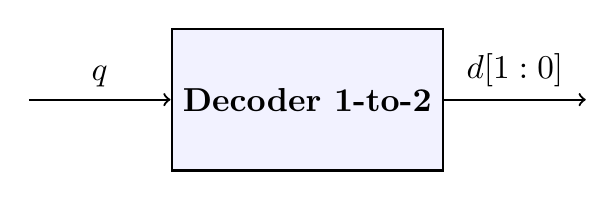
\begin{tikzpicture}[scale=1.2, transform shape]
    \node[draw, thick, fill=blue!5, minimum width=2.5cm, minimum height=1.5cm,
          align=center] (dec) {\textbf{Decoder 1-to-2}};

    \draw[->, thick] ([xshift=-1.5cm]dec.west) -- (dec.west)
        node[midway, above] {$q$};

    \draw[->, thick] (dec.east) -- ([xshift=1.5cm]dec.east)
        node[midway, above] {$d[1:0]$};
\end{tikzpicture}
\caption{Структурная схема дешифратора 1 в 2.}
\label{fig:decoder_1_to_2}
\end{figure}

\subsubsection{Использование конструкции \texttt{assign}}

В листинге \ref{lst:decoder_1_assign} представлена реализация дешифратора с использованием непрерывного присваивания. 

Конструкция \texttt{assign} применяется для описания \textit{комбинационной логики}. Особенностью данного подхода является то, что любые изменения на входе $q$ приводят к немедленному пересчёту и обновлению выходного значения $d$ без привязки к тактовым сигналам или фронтам.

\begin{code}
\caption{Реализация дешифратора через конструкцию \texttt{assign}.}
\label{lst:decoder_1_assign}
\begin{minted}{verilog}
module decoder_1_assign
(
    input wire q,
    output wire [1:0] d
);
    assign d = (q == 1'b0) ? 2'b01 : 2'b10;
endmodule
\end{minted}
\end{code}

\subsubsection{Использование \texttt{always}-блока}

В листинге \ref{lst:decoder_1_always} представлена альтернативная реализация дешифратора с использованием процедурного блока \texttt{always}.

Блок \texttt{always @(*)} также используется для описания \textit{комбинационной логики} из-за полного списка чувствительности \texttt{*}. Особенностью этой конструкции является процедурный стиль описания алгоритма, внутри которого допускается использование условных операторов и ветвлений для формирования выходного сигнала.

\begin{code}
\caption{Реализация дешифратора через \texttt{always}-блок.}
\label{lst:decoder_1_always}
\begin{minted}{verilog}
module decoder_1_always
(
    input wire q,
    output reg [1:0] d
);
    always @(*) begin
        d = (q == 1'b0) ? 2'b01 : 2'b10;
    end
endmodule
\end{minted}
\end{code}

\subsection{Разработка параметризируемого модуля}

\subsubsection{Идея переиспользования разработанного БОЭ}

Построение параметрического дешифратора размерности $N$ (где $N = 2^K$, а $K = \lceil\log_2 N\rceil$) на основе разработанного дешифратора «1-в-2» \textbf{невозможно}. К примеру, для создания дешифратора «2-к-4» необходимо, чтобы исходный дешифратор «1-в-2» мог подать на выход два нулевых бита, что противоречит его описанию.

Значит, для построения параметрического дешифратора необходимо изменить исходный БОЭ, добавив в него вход \texttt{enable}:
\begin{itemize}
    \item Если \texttt{enable} = 1, то дешифратор работает в обычном режиме.
    \item Если \texttt{enable} = 0, то на выходе формируется нулевой вектор.
\end{itemize}

На рисунке \ref{fig:decoder_2_to_4} представлена концептуальная схема иерархического построения дешифратора «2-в-4» из двух БОЭ «1-в-2».

\begin{figure}[!hbp]
\centering
\begin{tikzpicture}[
    scale=1.0, transform shape,
    blockMSB/.style={draw, thick, fill=blue!5, align=center,
                     minimum width=2.5cm, minimum height=2cm},
    blockLSB/.style={draw, thick, fill=green!5, align=center,
                     minimum width=2.5cm, minimum height=1.5cm},
    dot/.style={circle, fill=black, inner sep=0pt, minimum size=3pt},
    dotW/.style={dot, fill=white, draw=black, thick}
]
    \node[blockLSB, anchor=west] (dec21)
        at (1.5cm, 0.75cm)
        {\textbf{БОЭ 1}\\ \small\texttt{decoder\_1}};

    \node[blockLSB, anchor=north] (dec20)
        at ([yshift=-1cm]dec21.south)
        {\textbf{БОЭ 0}\\ \small\texttt{decoder\_1}};
    
    \coordinate (dec1) at ([xshift=-1.5cm]dec20.south);
    \draw[->, thick] ([xshift=-1.5cm]dec20.west |- dec1) |- coordinate (c1) (dec20.-200) node[pos=0, below] {$q[1]$} node[pos=1, above left] {$e$};
    \draw[->, thick] ([xshift=-0.75cm]dec20.west |- dec1) |- coordinate (c2) (dec20.-160) node[pos=0, below] {$q[0]$} node[pos=1, above left] {$q$};

    \draw[->, thick] (c1) |- (dec21.-200) node[pos=1, above left] {$e$};
    \draw[->, thick] (c2) |- (dec21.-160) node[pos=1, above left] {$q$};

    \node[dot, anchor=center] at (c1) {};
    \node[dot, anchor=center] at (c2) {};

    \node[dotW, anchor=center] at (dec20.-200) {};

    \draw[->, thick] ([yshift= 0.35cm]dec21.east) -- ++(1cm,0) node[right] {$d[3]$};
    \draw[->, thick] ([yshift=-0.35cm]dec21.east) -- ++(1cm,0) node[right] {$d[2]$};

    \draw[->, thick] ([yshift= 0.35cm]dec20.east) -- ++(1cm,0) node[right] {$d[1]$};
    \draw[->, thick] ([yshift=-0.35cm]dec20.east) -- ++(1cm,0) node[right] {$d[0]$};
\end{tikzpicture}
\caption{Структурная схема двухступенчатого дешифратора 2 в 4.}
\label{fig:decoder_2_to_4}
\end{figure}

\subsubsection{Реализация параметризируемого модуля}

В листинге \ref{lst:decoder_2_parametric} приведена реализация параметризируемого дешифратора с применением \texttt{generate}-блока.

\begin{code}
\caption{Параметризируемый дешифратор.}
\label{lst:decoder_2_parametric}
\begin{minted}{verilog}
module decoder_2_tuned
(
    input wire q, enable,
    output reg [1:0] d
);
    wire [1:0] decoder_d;
    decoder_1_assign decoder_1_to_2(q, decoder_d);
    assign d = ~enable ? 2'b00 : decoder_d;
endmodule

module decoder_tree
#(
    parameter int N = 2
)
(
    input wire enable,
    input wire [$clog2(N)-1:0] q,
    output wire [N-1:0] d
);
    generate
        if (N == 2) begin : g_leaf
            decoder_2_tuned u (
                .q(q[0]),
                .enable(enable),
                .d(d)
            );
        end else begin : g_node
            int MSB = $clog2(N) - 1;
            
            decoder_tree #(.N(N/2)) u_lo (
                .enable(enable & ~q[MSB]),
                .q(q[MSB-1:0]),
                .d(d[N/2-1:0])
            );
            decoder_tree #(.N(N/2)) u_hi (
                .enable(enable & q[MSB]),
                .q(q[MSB-1:0]),
                .d(d[N-1:N/2])
            );
        end
    endgenerate
endmodule
\end{minted}
\end{code}

\subsection{Разработка последовательного элемента}

Для сохранения значений и организации синхронной работы с тактовым сигналом разработан последовательный элемент \texttt{result\_keeper}, код которого представлен в листинге \ref{lst:result_keeper}.

\begin{code}
\caption{Модуль сохранения результата.}
\label{lst:result_keeper}
\begin{minted}{verilog}
module result_keeper
#(
    parameter int N = 2
)
(
    input wire clk, rst,
    input wire [N-1:0] q
);
    reg [N-1:0] result = 0;
    always @(posedge clk) begin
        if (~rst)
            result <= 0;
        else
            result <= q;
    end
endmodule
\end{minted}
\end{code}

\subsection{Тестирование разработанного элемента}

Для проверки корректности разработанных компонентов использовался \texttt{testbench}, который был интегрирован в среду проектирования. В тестах последовательно проверяются оба варианта простейших дешифраторов, параметрический дешифратор при $N=8$, а также логика работы элемента хранения данных с учетом тактирования и сигналов сброса. 

Код тестбенча вынесен в отдельный листинг в приложении \ref{sec:testbench_listing} ввиду его объёма. В приложении \ref{sec:sim_results} приведены результаты симуляции, которые подтверждают корректность работы всех разработанных модулей.

Данные симуляции полностью совпадают с ожидаемыми значениями:
\begin{itemize}
    \item Простейшие дешифраторы корректно декодируют входной сигнал в соответствии с таблицей истинности.
    \item Параметрический дешифратор успешно формирует позиции единиц для всех перебираемых индексов в диапазоне от $0$ до $N-1$.
    \item Элемент сохранения стабильно фиксирует входные данные по положительному фронту тактового сигнала \texttt{clk}, корректно сбрасывает накопленное значение при активном сигнале \texttt{rst} и возобновляет запись после его снятия.
\end{itemize}